\section{Design of fishtrap}
\label{sec:design}

We evaluated fishtrap version 1.0.0, which combines principles in \texttt{AGENTS.md} with five command hooks implemented by one Python script. The principles guide task interpretation; the hooks recall it at the events identified in the field study (Figure~\ref{fig:overview}). The evaluation tests each layer separately and together.

\subsection{Principles with reasons and a recipient}

The principles ask the agent to identify the desired end state and who will judge it. Counts, required fields, and size limits become constraints within that goal. An unattainable count calls for reporting the shortfall; a validation warning calls for checking the row's purpose and placement.

Each rule carries its purpose and scope. Concise chat serves a reader skimming on a phone; a requested document needs space for its content. Exact identifiers retain the form required to match them. Naming files for their recipient extends to substitute photos and later revisions. Reasons are intended to limit over-application and support application to new cases. Earlier agent-written precautions are working assumptions whose relevance follows the latest user instruction.

The recipient model covers filenames, attachments, fields, and messages: what does this reader need, and what does each item communicate? Process explanations and assumptions have an outlet in the report to the user. The destination's information requirements determine the submitted disclosures.

\subsection{Checks at the decision point}

More than 100 tool calls separate the initial instructions from the motivating uploads. Earlier correct behavior can coexist with a later failure. fishtrap schedules reminders at observable triggers (Table~\ref{tab:hooks}), using Codex event payloads and model-visible feedback \citep{openai2026hooks}. Matchers cover browser JavaScript calls through the Model Context Protocol (MCP), shell commands, and selected file patches; regular expressions detect outbound actions and validation messages. The \texttt{SessionStart} hook handles compaction, which replaces earlier conversation content with a summary, and session resumption.

\begin{table}[tb]
    \centering
    \small
    \setlength{\tabcolsep}{4pt}
    \caption{Five fishtrap hook registrations and their model-facing checks. One \texttt{PreToolUse} handler covers upload and submit/send.}
    \label{tab:hooks}
    \begin{tabularx}{\linewidth}{@{}l p{0.29\linewidth} X@{}}
        \toprule
        Event & Trigger & What the model is asked \\
        \midrule
        \texttt{UserPromptSubmit} & A later prompt adds a count, continues, or unblocks work. & What original criteria govern this request, and which parked items can now proceed? \\
        \texttt{SessionStart} & Compaction or resume, with a stored brief. & What did the user ask for, and which earlier precautions are working assumptions? \\
        \texttt{PreToolUse} & Detected upload or submit/send attempt. & What filenames, contents, and field values will the recipient see, and what will they conclude? \\
        \texttt{PostToolUse} & A result contains a validation warning. & Does each flagged entry belong here and need to exist? Which rows should move or be deleted? \\
        \texttt{Stop} & At least 12 matched tool calls in a turn, or a detected outbound action. & What observed evidence establishes each requested outcome, and what parked work can now be finished? \\
        \bottomrule
    \end{tabularx}
\end{table}

Before upload, \texttt{PreToolUse} denies the first attempt at a gate, listing filenames and detected naming concerns. Before submit or send, it requests a readback. The model inspects, fixes, and retries. This \emph{deny-once} design gives the check a turn before execution and leaves judgment with the model: an identical retry can proceed. Flagged filename sets have separate upload gates; clean names share a gate. Gates become eligible again after 40 matched calls for uploads and 20 for submissions; validation reminders have a 15-call interval. The closure check blocks once per substantial turn and uses \texttt{stop\_hook\_active} to prevent a loop.

\begin{figure}[tb]
    \centering
    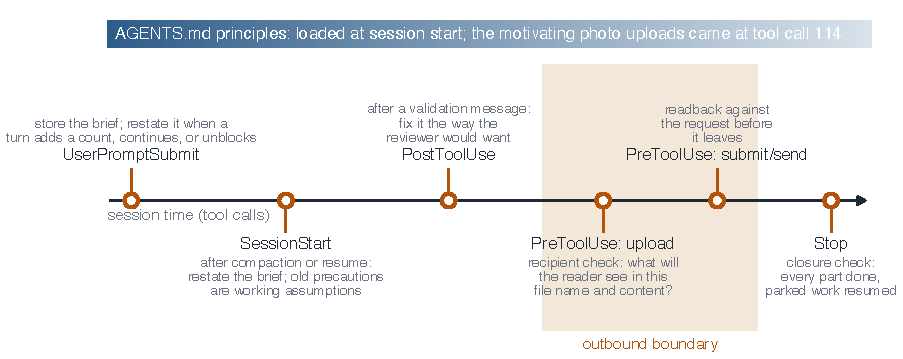
\includegraphics[width=\linewidth]{figs/overview.pdf}
    \caption{Schematic session timeline. Five event handlers cover the decision points; \texttt{PreToolUse} appears twice. Principles load at session start; the motivating photo uploads occurred at tool call 114.}
    \label{fig:overview}
\end{figure}

\subsection{Local operation and agent-driven installation}

The hooks use the Python standard library, make no network requests, and keep state and logs locally. They fail open on malformed input or internal errors. Coverage follows the recognized tool patterns. The model decides whether the recipient check warrants a change.

In version 1.0.0, when a user says ``install fishtrap,'' the agent follows \texttt{INSTALL.md} and runs \texttt{install.py} with their preferred name and optional profile path. The installer backs up configuration, inserts a marked principle block, merges five hook registrations, and runs an upload self-test. A person reviews and trusts the hooks through Codex's hook interface, then starts a new session. Re-running the installer updates its marked additions. Version 1.1.0 installs principles by default and adds revised hooks with \texttt{--hooks}; the hook revisions are unevaluated.
